\providecommand{\qcor}[1]{\ulcorner#1\urcorner}   %
\providecommand{\cellpair}[5]{$\vcenter{\hbox{\begin{tikzpicture}[x=1.15em,y=1.15em]%
\node (s) at (0,0) {$#1$};%
\node (t) at (4.2,0) {$#2$};%
\draw[->] (0.75,0.32) to[bend left=18] (3.45,0.32);%
\node at (2.1,0.88) {$\scriptstyle#3$};%
\draw[->] (0.75,-0.32) to[bend right=18] (3.45,-0.32);%
\node at (2.1,-0.93) {$\scriptstyle#4$};%
\draw[->] (1.95,0.2) to[bend right=32] (1.95,-0.2);%
\node at (2.85,0) {$\scriptstyle#5$};%
\end{tikzpicture}}}$\ignorespaces}

\section{离散笛卡尔纤维化}\label{sec:discrete-cartesian-fibrations}

\trCartesianFibration{}与余笛卡尔纤维化编码了这样一些\trInfinityCategory{}族：%
它们被底∞-范畴反变地或协变地作用。
在某些特殊情形，作为\trCartesianFibration{}或余笛卡尔纤维化的诸\trFiber{}而%
出现的那些\trInfinityCategory{}都是\emph{\trDiscrete}（见定义 1.2.26）。
由于 1-范畴之间的类似函子被称为\emph{离散纤维化}（discrete fibration）与%
\emph{离散余纤维化}（discrete opfibration），我们把这些\trInfinityCategory{}%
之间的映射分别称作
「\trDiscreteCartesianFibration」与「\trDiscreteCocartesianFibration」。本节的目的便是研究这一特殊的%
\trFibration{}类。

在给出定义之前，我们先来描述一条\trIsofibration{} $p\colon E\twoheadrightarrow B$
所需要的那种合适的「离散性」。回忆练习 1.4.iv：\trInfinityCosmos{} $\mathcal{K}$
中的一个对象 $E$ 是\textbf{\trDiscrete}，当且仅当余定义域为 $E$ 的每个自然变换%
都可逆。
离散纤维化是\trInfinityCosmos{} $\mathcal{K}$ 中那些视为\trSliceInfinityCosmos{}
$\mathcal{K}_{/B}$ 的对象时为离散的\trIsofibration{} $p\colon E\twoheadrightarrow B$；
我们简称这类映射为\textbf{离散等价纤维化}（discrete isofibration）。
借助命题 3.6.2，有多种彼此等价的方式可以在\trHomotopyTwoCategory{}
$\hbar\mathcal{K}$ 的层面上把 $\mathcal{K}_{/B}$ 中离散对象这一概念展开：

\begin{lemma}\label{lem:discrete-isofibration-characterizations}
一条\trIsofibration{} $p\colon E\twoheadrightarrow B$ 是离散等价纤维化，当且仅%
当下列%
两组等价条件中的任何一组成立：
\begin{enumerate}[label=(\roman*)]
\item 任何使 $p\psi$ 为恒同的 2-胞腔
\cellpair{X}{E}{a}{b}{\psi}
皆可逆。
\item 任何使 $p\psi$ 为一个\trIsomorphism{}的 2-胞腔
\cellpair{X}{E}{a}{b}{\psi}
皆可逆。
\end{enumerate}
\end{lemma}

\begin{proof}
\cref{ex:prove-discrete-isofibration-lemma}。
\end{proof}

于是，离散等价纤维化恰好就是那些在\trHomotopyTwoCategory{}中定义保守函子的%
\trIsofibration。
一条离散等价纤维化的定义域与余定义域都无须是离散的\trInfinityCategory{}（见%
\cref{ex:discreteness-exploration}）。毋宁说，\trSliceInfinityCosmos{}中的%
离散性是「逐纤维的」。

\begin{lemma}\label{lem:discrete-isofibration-fibers}
离散等价纤维化的诸\trFiber{}都是离散的\trInfinityCategory。
\end{lemma}

\begin{proof}
回忆注 1.3.3：离散的\trInfinityCategory{}被\trCosmologicalFunctor{}保持。
特别地，与\trElement{} $b\colon 1\to B$ 相关联的\trPullback{}函子
$b^{*}\colon\mathcal{K}_{/B}\to\mathcal{K}$ 保持离散对象。于是，离散等价纤维化
$p\colon E\twoheadrightarrow B$ 的诸\trFiber{}都是离散的\trInfinityCategory。
\end{proof}

\cref{lem:discrete-isofibration-fibers}之逆在 $(\infty,1)$-范畴的%
\trInfinityCosmos{}中成立：$(\infty,1)$-范畴之间的一条\trIsofibration{}
$p\colon E\twoheadrightarrow B$ 是离散的，当且仅当它的诸\trFiber{}是离散的%
\trInfinityCategory{}（见命题 12.2.3）。
于是，在这类\trInfinityCosmos{}中，我们即将引入的\trDiscreteCartesianFibration{}与\trDiscreteCocartesianFibration{}可以
理解为具有离散\trFiber{}的\trCartesianFibration。

\begin{definition}[离散余/笛卡尔纤维化]\label{def:discrete-co-cartesian-fibration}
\trInfinityCosmos{} $\mathcal{K}$ 中的一条\trIsofibration{}
$p\colon E\twoheadrightarrow B$
是\textbf{\trDiscreteCartesianFibration}（discrete cartesian fibration），若它是一条%
\trCartesianFibration{}且作为 $\mathcal{K}_{/B}$ 的对象为离散。对偶地，$p$
是\textbf{\trDiscreteCocartesianFibration}（discrete cocartesian fibration），若它是一条%
余笛卡尔纤维化且作为 $\mathcal{K}_{/B}$ 的对象为离散。
\end{definition}

\begin{digression}[拟范畴的\trLeftFibration{}与\trRightFibration]\label{dig:left-right-fibrations}
在\trQuasiCategory{}的\trInfinityCosmos{}中，\trDiscreteCocartesianFibration{}与 Joyal 的%
\textbf{\trLeftFibration}（left fibration）类——即那些相对于左号角包含具有提升性质的%
映射——相重合；
对偶地，\trDiscreteCartesianFibration{}与 Joyal 的\textbf{\trRightFibration}（right fibration）类相重合
（见命题 F.4.9）。
虽然\trLeftFibration/\trRightFibration{}的术语在\trInfinityCategory{}论的文献中更为人熟悉，我们仍使用%
「离散余/笛卡尔%
纤维化」这些术语，以厘清这些映射类与它们的非离散类比以及 1-范畴类比之间的关系。
\end{digression}

如 5.4 节中那样，\trDiscreteCocartesianFibration{}的理论可以通过在\trCodualInfinityCosmos{}中%
解释关于\trDiscreteCartesianFibration{}的结果而得到，所以我们把注意力集中于\trDiscreteCartesianFibration%
这一类上，以精简行文。

\begin{lemma}[拉回稳定性]\label{lem:discrete-pullback-stability}
在任何\trPullback{}方块
\begin{center}
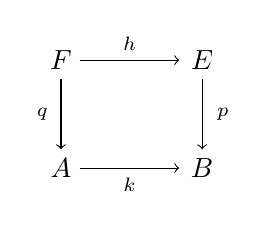
\begin{tikzpicture}[x=1.5em,y=1.5em]
  \node (F) at (0,1.3) {$F$};
  \node (E) at (3.4,1.3) {$E$};
  \node (A) at (0,-1.3) {$A$};
  \node (B) at (3.4,-1.3) {$B$};
  \draw[->] (0.45,1.3) -- node[above]{$\scriptstyle h$} (2.85,1.3);
  \draw[->] (0.45,-1.3) -- node[below]{$\scriptstyle k$} (2.85,-1.3);
  \draw[->] (0,0.85) -- (0,-0.85);
  \node at (-0.45,0) {$\scriptstyle q$};
  \draw[->] (3.4,0.85) -- (3.4,-0.85);
  \node at (3.9,0) {$\scriptstyle p$};
  \node at (0.45,0.85) {$\scriptstyle\llcorner$};
\end{tikzpicture}
\end{center}
中，若 $p$ 是一条\trDiscreteCartesianFibration，则 $q$ 亦是一条\trDiscreteCartesianFibration。
\end{lemma}

\begin{proof}
有命题 5.2.4 在手，只剩下验证 $q$ 是离散的。
考虑一个使 $q\psi$ 可逆的 2-胞腔
\cellpair{X}{F}{a}{b}{\psi}。
于是 $kq\psi=ph\psi$ 可逆，而 $p$ 的保守性蕴含 $h\psi$ 可逆。
由\trTwoCellConservativity{}（见命题 3.3.1），$\psi$ 也可逆。
\footnote{原书印作「$\gamma$ 也可逆」，但本证明中并无 $\gamma$，显系 $\psi$
之误，此处径改。——译者注}
\end{proof}

\trDiscreteCartesianFibration{}存在一个直接的 2-范畴式刻画，即把它刻画为那些具有如下性质的%
\trIsofibration{} $p\colon E\twoheadrightarrow B$：余定义域为 $pe$ 的每个%
\trNaturalTransformation{} $\beta\colon b\Rightarrow pe$ 都容有一个本质唯一的、
余定义域为 $e$ 的\trLifting。
这与下述观察紧密相关：对于\trDiscreteCartesianFibration{} $p$ 而言，不存在特殊的 $p$-笛卡尔%
箭头类——非离散版本的情形则不然。

\begin{proposition}\label{prop:discrete-cartesian-characterization}
\begin{enumerate}[label=(\roman*)]
\item 若 $p\colon E\twoheadrightarrow B$ 是一条\trDiscreteCartesianFibration，则余定义域为 $E$
的每个\trNaturalTransformation{}都是 $p$-\trCartesian。
\item 一条\trIsofibration{} $p\colon E\twoheadrightarrow B$ 是\trDiscreteCartesianFibration，
当且仅当余定义域为 $pe$ 的每个\trNaturalTransformation{} $\beta\colon b\Rightarrow pe$
都容有一个本质唯一的、余定义域为 $e$ 的\trLifting：给定 $\chi\colon e'\Rightarrow e$
与 $\psi\colon e''\Rightarrow e$ 使得 $p\chi=p\psi=\beta$，则存在一个%
\trIsomorphism{} $\gamma\colon e''\Rightarrow e'$ 使得 $\chi\cdot\gamma=\psi$
且 $p\gamma=\mathrm{id}$。
\end{enumerate}
\end{proposition}

\begin{proof}
由命题 5.1.13，若 $p\colon E\twoheadrightarrow B$ 是一条\trCartesianFibration，
则余定义域为 $E$ 的任何\trNaturalTransformation{} $\psi$ 都经由一个使
$p\gamma=\mathrm{id}$ 的\trNaturalTransformation{} $\gamma$，穿过 $p\psi$ 的某个
$p$-笛卡尔提升而分解。
当 $p$ 离散时，这个 $\gamma$ 是一个\trIsomorphism，于是 $\psi$ 同构于一条
$p$-笛卡尔变换，从而由引理 5.1.6，它本身也是 $p$-\trCartesian。

由 (i) 中刚刚观察到的结论与引理 5.1.11 中 $p$-笛卡尔提升的本质唯一性可见：若
$p\colon E\twoheadrightarrow B$ 是一条\trDiscreteCartesianFibration，则任何%
\trNaturalTransformation{} $\beta\colon b\Rightarrow pe$ 都容有一个本质唯一的%
\trLifting。
反之，注意任何满足 (ii) 之假设的 $p\colon E\twoheadrightarrow B$ 都是一条离散%
等价纤维化：若 $\psi\colon e'\Rightarrow e$ 使得 $p\psi=\mathrm{id}$，则
$\mathrm{id}\colon e\Rightarrow e$ 是 $p\psi$ 的另一个\trLifting，而本质唯一性%
提供了%
一个逆\trIsomorphism{} $\psi^{-1}\colon e\Rightarrow e'$。

为完成证明，还需证：任何满足 (ii) 之假设的 $p\colon E\twoheadrightarrow B$ 都是%
一条\trCartesianFibration。我们通过建立命题 5.2.11 的 2-范畴式刻画来做到这一点，
即证明：余定义域为 $E$ 的任何 2-胞腔 $\psi\colon e'\Rightarrow e$ 都是弱
$p$-\trCartesian——从而再由命题 5.2.11，它按通常的意义是 $p$-\trCartesian。
为此，考虑一对 $\tau\colon e''\Rightarrow e$ 与 $\gamma\colon pe''\Rightarrow pe'$，
使得 $p\tau=p\psi\cdot\gamma$。由「每个 2-胞腔都容许本质唯一\trLifting」这一%
假设，我们
可以构造一个\trLifting{} $\mu\colon\bar{e}\Rightarrow e'$，使得 $p\mu=\gamma$。现在 $\tau$
与 $\psi\cdot\mu$ 是 $p\tau$ 的两个具有相同余定义域的\trLifting，故存在一个%
\trIsomorphism{} $\zeta\colon e''\Rightarrow\bar{e}$，使得 $p\zeta=\mathrm{id}$。
复合 $\mu\cdot\zeta$ 便定义了 $\gamma$ 到某个胞腔的所欲\trLifting，使得
$\tau=\psi\cdot\mu\cdot\zeta$。
\end{proof}

作为 (i) 的一个直接推论：

\begin{corollary}\label{cor:square-into-discrete-cartesian}
从一条\trCartesianFibration{}到一条\trDiscreteCartesianFibration{}的任何交换方块都定义一个%
\trCartesianFunctor。
\end{corollary}

与定理 5.2.8 相类似，\trDiscreteCartesianFibration{}也有一个内部刻画，而它在离散情形下取一个%
简单得多的形式。

\begin{proposition}[\trDiscreteCartesianFibration{}的内部刻画]\label{prop:internal-characterization-discrete}
一条\trIsofibration{} $p\colon E\twoheadrightarrow B$ 是\trDiscreteCartesianFibration，当且%
仅当函子
$i_{1}\hat{p}\colon E^{2}\twoheadrightarrow\mathrm{Hom}_{B}(B,p)$ 是一个%
\trTrivialFibration。
\end{proposition}

回忆定理 5.2.8(ii)：一条\trIsofibration{} $p\colon E\twoheadrightarrow B$ 定义%
一条%
\trCartesianFibration，当且仅当
$i_{1}\hat{p}\colon E^{2}\twoheadrightarrow\mathrm{Hom}_{B}(B,p)$ 容有一个%
右伴随右逆 $\qcor{\chi}$。
\cref{prop:internal-characterization-discrete}宣称：$p$ 定义一条\trDiscreteCartesianFibration，当且仅当这一伴随定义一个%
\trAdjointEquivalence。

\begin{proof}
首先假设 $p\colon E\twoheadrightarrow B$ 是一条\trDiscreteCartesianFibration。由定理
5.2.8(ii)，$i_{1}\hat{p}\colon E^{2}\to\mathrm{Hom}_{B}(B,p)$ 便容有一个带可逆%
余单位 $\bar{\epsilon}\colon(i_{1}\hat{p})\qcor{\chi}\cong\mathrm{id}$ 的右伴随
$\qcor{\chi}$。我们要论证：此时单位 $\bar{\eta}\colon\mathrm{id}\Rightarrow\qcor{\chi}(i_{1}\hat{p})$ 也可逆，从而证明 $i_{1}\hat{p}\dashv\qcor{\chi}$
定义一个\trAdjointEquivalence。

由于 $i_{1}\hat{p}\dashv\qcor{\chi}$ 的余单位可逆，$(i_{1}\hat{p})\bar{\eta}$
是一个\trIsomorphism。于是 $p_{1}(i_{1}\hat{p})\bar{\eta}=p_{1}\bar{\eta}$ 与
$p_{0}(i_{1}\hat{p})\bar{\eta}=pp_{0}\bar{\eta}$ 都是\trIsomorphism。由%
\cref{lem:discrete-isofibration-characterizations}所证明的离散纤维化
$p\colon E\twoheadrightarrow B$ 的保守性，这蕴含 $p_{0}\bar{\eta}$ 可逆；再用
$E^{2}$ 的\trTwoCellConservativity{}即见 $\bar{\eta}$ 是一个\trIsomorphism。

反之，若 $i_{1}\hat{p}\colon E^{2}\twoheadrightarrow\mathrm{Hom}_{B}(B,p)$
是一个\trTrivialFibration，则由命题 2.1.12 与引理 3.6.9，我们可以选取一个%
右伴随右逆\trEquivalence{} $\qcor{\chi}\colon\mathrm{Hom}_{B}(B,p)\twoheadrightarrow E^{2}$。
与 $\qcor{\chi}$ 复合即见：任何箭头 $\qcor{\beta}\colon X\to\mathrm{Hom}_{B}(B,p)$
都容有一个\trLifting。这一\trAdjointEquivalence{}的单位必然是一个%
\trFiberedIsomorphism，于是对任何箭头 $\qcor{\psi}\colon X\to E^{2}$ 我们有一条%
粘贴等式
\begin{center}
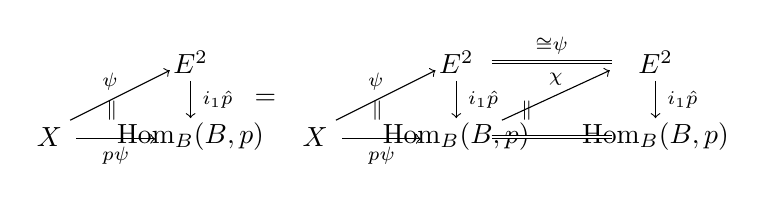
\begin{tikzpicture}[x=1.5em,y=1.5em]
  \node (X1) at (0,0) {$X$};
  \node (E1) at (3.4,1.8) {$E^{2}$};
  \node (H1) at (3.4,0) {$\mathrm{Hom}_{B}(B,p)$};
  \draw[->] (0.5,0.4) -- node[above,pos=0.4]{$\scriptstyle\qcor{\psi}$} (2.9,1.6);
  \node at (1.5,0.62) {$\scriptstyle\parallel$};
  \draw[->] (0.65,-0.05) -- (2.55,-0.05);
  \node at (1.6,-0.45) {$\scriptstyle\qcor{p\psi}$};
  \draw[->] (3.4,1.35) -- (3.4,0.45);
  \node at (4.05,0.9) {$\scriptstyle i_{1}\hat{p}$};
  \node at (5.2,0.9) {$=$};
  \begin{scope}[shift={(6.4,0)}]
  \node (X2) at (0,0) {$X$};
  \node (E2) at (3.4,1.8) {$E^{2}$};
  \node (E3) at (8.2,1.8) {$E^{2}$};
  \node (H2) at (3.4,0) {$\mathrm{Hom}_{B}(B,p)$};
  \node (H3) at (8.2,0) {$\mathrm{Hom}_{B}(B,p)$};
  \draw[->] (0.5,0.4) -- node[above,pos=0.4]{$\scriptstyle\qcor{\psi}$} (2.9,1.6);
  \node at (1.5,0.62) {$\scriptstyle\parallel$};
  \draw[->] (0.65,-0.05) -- (2.55,-0.05);
  \node at (1.6,-0.45) {$\scriptstyle\qcor{p\psi}$};
  \draw[->] (3.4,1.35) -- (3.4,0.45);
  \node at (4.05,0.9) {$\scriptstyle i_{1}\hat{p}$};
  \draw[double] (4.25,1.8) -- (7.15,1.8);
  \node at (5.7,2.2) {$\scriptstyle\cong\qcor{\psi}$};
  \draw[double] (4.25,0) -- (7.15,0);
  \draw[->] (4.5,0.4) -- node[above,pos=0.5]{$\scriptstyle\qcor{\chi}$} (7.1,1.6);
  \node at (5.1,0.62) {$\scriptstyle\parallel$};
  \draw[->] (8.2,1.35) -- (8.2,0.45);
  \node at (8.85,0.9) {$\scriptstyle i_{1}\hat{p}$};
  \end{scope}
\end{tikzpicture}
\end{center}
由于右边的图是一个绝对右提升图表，左边亦然；于是由定理 5.1.7(ii) 我们断定：余%
定义域为 $E$ 的每支箭头都是 $p$-\trCartesian。
现在，引理 5.1.6 中\trCartesianArrow{}的保守性性质适用于所有箭头，并告诉我们
$p\colon E\twoheadrightarrow B$ 定义一个保守函子，从而特别地是离散的。
\end{proof}

作为\cref{prop:internal-characterization-discrete}的一个推论，显然%
\trCosmologicalFunctor{}保持\trDiscreteCartesianFibration。利用这一内部刻画，验证\trDiscreteCartesianFibration{}可以复合且可以左消去也是直截了当的：

\begin{lemma}\label{lem:discrete-cartesian-cancellation}
设 $p\colon E\twoheadrightarrow B$ 与 $q\colon B\twoheadrightarrow A$
为\trIsofibration，且 $q$ 是一条\trDiscreteCartesianFibration。则 $p$ 是\trDiscreteCartesianFibration，
当且仅当 $qp$ 是\trDiscreteCartesianFibration。
\end{lemma}

\begin{proof}
检测 $qp\colon E\twoheadrightarrow A$ 是否\trDiscreteCartesianFibration{}的那个映射
$E^{2}\twoheadrightarrow\mathrm{Hom}_{A}(A,qp)$ 可以因子分解为：先经过检测
$p\colon E\twoheadrightarrow B$ 是否\trDiscreteCartesianFibration{}的映射
$E^{2}\twoheadrightarrow\mathrm{Hom}_{B}(B,p)$，再经过检测
$q\colon B\twoheadrightarrow A$ 是否\trDiscreteCartesianFibration{}的映射
$B^{2}\twoheadrightarrow\mathrm{Hom}_{A}(A,q)$ 的一个\trPullback：
\begin{center}
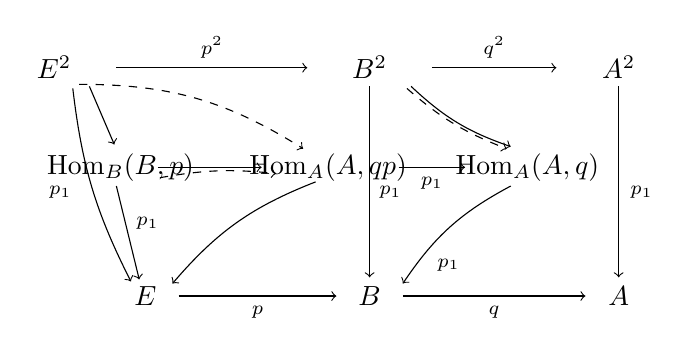
\begin{tikzpicture}[x=1.5em,y=1.5em]
  \node (E2)  at (0,4.6) {$E^{2}$};
  \node (B2)  at (7.6,4.6) {$B^{2}$};
  \node (A2)  at (13.6,4.6) {$A^{2}$};
  \node (HB)  at (1.6,2.2) {$\mathrm{Hom}_{B}(B,p)$};
  \node (HAB) at (6.6,2.2) {$\mathrm{Hom}_{A}(A,qp)$};
  \node (HAQ) at (11.4,2.2) {$\mathrm{Hom}_{A}(A,q)$};
  \node (E)   at (2.2,-0.9) {$E$};
  \node (B)   at (7.6,-0.9) {$B$};
  \node (A)   at (13.6,-0.9) {$A$};
  \draw[->] (1.5,4.6) -- node[above]{$\scriptstyle p^{2}$} (6.1,4.6);
  \draw[->] (9.1,4.6) -- node[above]{$\scriptstyle q^{2}$} (12.1,4.6);
  \draw[->,dashed] (0.6,4.2) to[bend left=16] (6.0,2.65);
  \draw[->] (0.85,4.15) -- (1.45,2.75);
  \draw[->] (2.5,2.2) -- (5.0,2.2);
  \node at (2.65,1.75) {$\scriptstyle\llcorner$};
  \draw[->,dashed] (2.55,1.95) to[bend left=8] (5.35,2.05);
  \draw[->] (8.3,2.2) -- node[below]{$\scriptstyle p_{1}$} (9.9,2.2);
  \draw[->] (8.6,4.15) to[bend right=12] (11.0,2.7);
  \node at (9.3,3.1) {$\scriptstyle\llcorner$};
  \draw[->,dashed] (8.5,4.1) to[bend right=10] (10.9,2.65);
  \draw[->] (0.45,4.1) to[bend right=10] (1.85,-0.55);
  \node at (0.15,1.6) {$\scriptstyle p_{1}$};
  \draw[->] (1.5,1.75) -- (2.05,-0.5);
  \node at (2.25,0.85) {$\scriptstyle p_{1}$};
  \draw[->] (6.3,1.85) to[bend right=14] (2.85,-0.6);
  \draw[->] (7.6,4.15) -- (7.6,-0.45);
  \node at (8.1,1.6) {$\scriptstyle p_{1}$};
  \draw[->] (13.6,4.15) -- (13.6,-0.45);
  \node at (14.15,1.6) {$\scriptstyle p_{1}$};
  \draw[->] (11.0,1.75) to[bend right=14] (8.4,-0.6);
  \node at (9.5,-0.15) {$\scriptstyle p_{1}$};
  \draw[->] (3.0,-0.9) -- node[below]{$\scriptstyle p$} (6.8,-0.9);
  \draw[->] (8.4,-0.9) -- node[below]{$\scriptstyle q$} (12.8,-0.9);
\end{tikzpicture}
\end{center}
此结果现在由引理 1.2.14 与等价的\trTwoOfThreeProperty{}得出。
\end{proof}

现在我们转向\trDiscreteCartesianFibration{}的若干例子。

\begin{lemma}\label{lem:trivial-fibration-discrete-bifibration}
一条\trTrivialFibration{} $p\colon E\twoheadrightarrow B$ 是一个离散\trBifibration。
\end{lemma}

\begin{proof}
由引理 1.2.14，$i_{1}\hat{p}\colon E^{2}\twoheadrightarrow\mathrm{Hom}_{B}(B,p)$
与 $i_{0}\hat{p}\colon E^{2}\twoheadrightarrow\mathrm{Hom}_{B}(p,B)$ 都是%
\trTrivialFibration。
于是\cref{prop:internal-characterization-discrete}及其对偶证明：$p$ 既是一条%
\trDiscreteCartesianFibration，也是一条\trDiscreteCocartesianFibration。
\end{proof}

本章开头处的讨论提示我们：对\trInfinityCategory{} $B$ 的任何\trElement{}
$b\colon 1\to B$，
右可表示 $p_{0}\colon\mathrm{Hom}_{B}(B,b)\twoheadrightarrow B$ 定义一条\trDiscreteCartesianFibration。
我们将在\cref{cor:domain-projection-from-element}中，把它作为关于第 II 部分之%
中心研究对象的一条更精细的观察的推论而导出。命题 5.2.9 证明：对任何%
\trInfinityCategory{} $A$，
定义域投影函子 $p_{0}\colon A^{2}\twoheadrightarrow A$ 定义一条%
\trCartesianFibration。
除非 $A$ 是离散的，这一函子并不定义一条\trDiscreteCartesianFibration（见%
\cref{ex:discreteness-exploration}）。然而，回忆 $p_{0}$-笛卡尔提升可以被构造得
使之沿 $p_{1}\colon A^{2}\twoheadrightarrow A$ 投影为恒同箭头。这提示我们：把%
定义域投影函子视为 $A$ 之上的一个映射来考虑或许富有成效；在此情形我们有如下结果。

\begin{proposition}\label{prop:domain-projection-sliced}
对\trInfinityCosmos{} $\mathcal{K}$ 中的任何\trInfinityCategory{} $A$，图表
\begin{rveq}\label{eq:domain-projection-over-A}
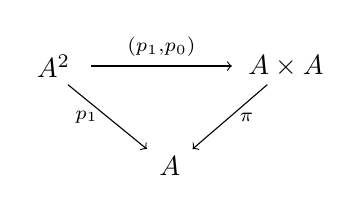
\begin{tikzpicture}[x=1.5em,y=1.5em]
  \node (A2) at (0,1.4) {$A^{2}$};
  \node (AA) at (5.6,1.4) {$A\times A$};
  \node (A)  at (2.8,-1.0) {$A$};
  \draw[->] (0.9,1.4) -- node[above]{$\scriptstyle(p_{1},p_{0})$} (4.3,1.4);
  \draw[->] (0.35,0.95) -- node[left,pos=0.5]{$\scriptstyle p_{1}$} (2.25,-0.6);
  \draw[->] (5.15,0.95) -- node[right,pos=0.5]{$\scriptstyle\pi$} (3.35,-0.6);
\end{tikzpicture}
\end{rveq}
在\trSliceInfinityCosmos{} $\mathcal{K}_{/A}$ 中定义一条\trDiscreteCartesianFibration。
\end{proposition}

\begin{proof}
由\trTwoCellConservativity，\eqref{eq:domain-projection-over-A} 是%
\trSliceInfinityCosmos{}
$(\mathcal{K}_{/A})_{/\pi\colon A\times A\twoheadrightarrow A}\cong\mathcal{K}_{/A\times A}$ 中的一个离散对象。于是只剩下证明这一函子定义一条%
\trCartesianFibration。我们利用定理 5.2.8(iii) 来证明这一点。
第一步是通过在\trSliceInfinityCosmos{} $\mathcal{K}_{/A}$ 中解释公式 (3.4.2)，
计算出函子 \eqref{eq:domain-projection-over-A} 的右可表示逗号对象。
由命题 1.2.22，对象 $\pi\colon A\times A\twoheadrightarrow A$ 的 2-余张量是
$\pi\colon A\times A^{2}\twoheadrightarrow A$，而这个右可表示逗号由下方
$\mathcal{K}_{/A}$ 中左手的\trPullback{}计算得出：
\begin{center}
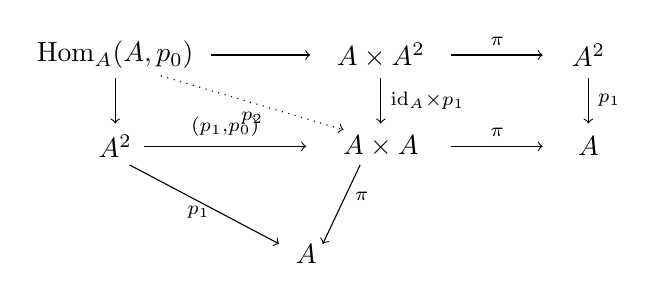
\begin{tikzpicture}[x=1.5em,y=1.5em]
  \node (HA)   at (0,3.4) {$\mathrm{Hom}_{A}(A,p_{0})$};
  \node (AXA2) at (6.4,3.4) {$A\times A^{2}$};
  \node (A2t)  at (11.4,3.4) {$A^{2}$};
  \node (A2m)  at (0,1.2) {$A^{2}$};
  \node (AXA)  at (6.4,1.2) {$A\times A$};
  \node (Am)   at (11.4,1.2) {$A$};
  \node (Ab)   at (4.6,-1.4) {$A$};
  \draw[->] (2.3,3.4) -- (4.7,3.4);
  \draw[->] (8.1,3.4) -- node[above]{$\scriptstyle\pi$} (10.3,3.4);
  \draw[->] (0,2.85) -- (0,1.75);
  \draw[->,dotted] (1.1,2.9) -- node[below,pos=0.5]{$\scriptstyle p_{2}$} (5.5,1.6);
  \node at (2.4,2.95) {$\scriptstyle\llcorner$};
  \draw[->] (0.7,1.2) -- node[above]{$\scriptstyle(p_{1},p_{0})$} (4.6,1.2);
  \draw[->] (8.1,1.2) -- node[above]{$\scriptstyle\pi$} (10.3,1.2);
  \draw[->] (6.4,2.85) -- node[right]{$\scriptstyle\mathrm{id}_{A}\times p_{1}$} (6.4,1.75);
  \draw[->] (11.4,2.85) -- node[right]{$\scriptstyle p_{1}$} (11.4,1.75);
  \draw[->] (0.35,0.75) -- node[left,pos=0.6]{$\scriptstyle p_{1}$} (3.95,-1.15);
  \draw[->] (5.9,0.75) -- node[right,pos=0.4]{$\scriptstyle\pi$} (5.0,-1.15);
\end{tikzpicture}
\end{center}
与 $\mathcal{K}$ 中右手的\trPullback{}作粘贴，我们便认出：如此构造的%
\trInfinityCategory{}与视为 $\mathcal{K}$ 中映射的函子
$p_{0}\colon A^{2}\twoheadrightarrow A$ 的右可%
表示逗号对象相重合。类似地，在 $\mathcal{K}$ 中由 $\mathrm{id}_{A}$ 诱导的典范%
函子 $\Delta_{p_{0}}\colon A^{2}\to\mathrm{Hom}_{A}(A,p_{0})$ 与在 $\mathcal{K}_{/A}$
中由 $\mathrm{id}_{(p_{1},p_{0})}$ 诱导的 $A$ 之上的典范函子
$\Delta_{(p_{1},p_{0})}\colon A^{2}\to\mathrm{Hom}_{A}(A,p_{0})$ 相重合。

在命题 5.2.9 的证明中所建立的\trIsomorphism{}
$\mathrm{Hom}_{A}(A,p_{0})\cong A^{3}$ 之下，\trIsofibration{}
$p_{2}\colon\mathrm{Hom}_{A}(A,p_{0})\twoheadrightarrow A$ 是在可复合箭头对的%
末元素 $2\in 3$ 处的求值。
由于 $p_{0}\colon A^{2}\twoheadrightarrow A$ 是 $\mathcal{K}$ 中的一条%
\trCartesianFibration，定理 5.2.8(iii) 告诉我们：函子
$\Delta_{p_{0}}\colon A^{2}\to\mathrm{Hom}_{A}(A,p_{0})\cong A^{3}$ 容有一个 $A$
之上的\trRightAdjoint{} $r$。命题 5.2.9 的证明与定理 5.2.8(ii)$\Rightarrow$(iii)
的证明（后者可以从定理 5.1.7(ii)$\Rightarrow$(iii) 的证明中抽取出来）相结合%
提供了一个构造：这一伴随可以通过把下左的诸范畴之复合伴随余张量入 $A$ 而定义：
\begin{center}
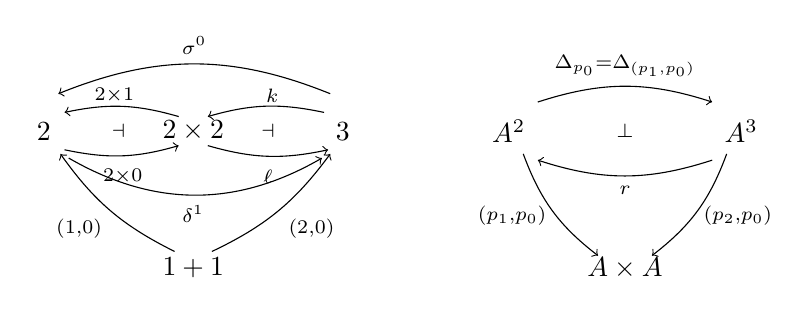
\begin{tikzpicture}[x=1.5em,y=1.5em]
  \node (two)   at (0,1.6) {$2$};
  \node (two2)  at (3.6,1.6) {$2\times 2$};
  \node (three) at (7.2,1.6) {$3$};
  \draw[->] (6.9,2.5) to[bend right=22] node[above]{$\scriptstyle\sigma^{0}$} (0.35,2.5);
  \draw[->] (3.25,1.95) to[bend right=14] (0.5,2.05);
  \node at (1.7,2.45) {$\scriptstyle 2\times 1$};
  \draw[->] (0.5,1.15) to[bend right=14] (3.25,1.25);
  \node at (1.9,0.5) {$\scriptstyle 2\times 0$};
  \node at (1.8,1.6) {$\scriptstyle\dashv$};
  \draw[->] (6.75,2.05) to[bend right=14] (3.95,1.95);
  \node at (5.5,2.45) {$\scriptstyle k$};
  \draw[->] (3.95,1.25) to[bend right=14] (6.85,1.15);
  \node at (5.4,0.5) {$\scriptstyle\ell$};
  \node at (5.4,1.6) {$\scriptstyle\dashv$};
  \node (one1) at (3.6,-1.7) {$1+1$};
  \draw[->] (3.15,-1.3) to[bend left=14] (0.4,1.05);
  \node at (0.85,-0.75) {$\scriptstyle(1,0)$};
  \draw[->] (4.05,-1.3) to[bend right=14] (6.9,1.05);
  \node at (6.45,-0.75) {$\scriptstyle(2,0)$};
  \draw[->] (0.6,0.95) to[bend right=30] (6.7,0.95);
  \node at (3.6,-0.4) {$\scriptstyle\delta^{1}$};
  \node at (9.6,1.6) {$\rightsquigarrow$};
  \begin{scope}[shift={(11.2,0)}]
  \node (A2) at (0,1.6) {$A^{2}$};
  \node (A3) at (5.6,1.6) {$A^{3}$};
  \draw[->] (0.7,2.3) to[bend left=18] node[above]{$\scriptstyle\Delta_{p_{0}}=\Delta_{(p_{1},p_{0})}$} (4.9,2.3);
  \node at (2.8,1.6) {$\scriptstyle\perp$};
  \draw[->] (4.9,0.9) to[bend left=18] node[below]{$\scriptstyle r$} (0.7,0.9);
  \node (AA) at (2.8,-1.7) {$A\times A$};
  \draw[->] (0.35,1.05) to[bend right=16] node[left,pos=0.55]{$\scriptstyle(p_{1},p_{0})$} (2.15,-1.4);
  \draw[->] (5.25,1.05) to[bend left=16] node[right,pos=0.55]{$\scriptstyle(p_{2},p_{0})$} (3.45,-1.4);
  \end{scope}
\end{tikzpicture}
\end{center}
其中 $\ell\dashv k$ 已在命题 5.2.9 的证明中描述。复合右伴随是函子
$\sigma^{0}\colon 3\to 2$，它把 $0$ 与 $1$ 送到 $0$、把 $2$ 送到 $1$；而复合左%
伴随是函子 $\delta^{1}\colon 2\to 3$，它把 $0$ 送到 $0$、把 $1$ 送到 $2$。特别地，
这一伴随位于「2 与 3 的『端点』之包含下」的严格切片 2-范畴中。
于是，余张量入 $A$ 后，我们得到 $A\times A$ 之上的一个\trFiberedAdjunction；由定理
5.2.8(iii)，这蕴含 \eqref{eq:domain-projection-over-A} 是 $\mathcal{K}_{/A}$ 中的%
一条\trCartesianFibration，证明完成。
\end{proof}

把命题 5.2.9 与\cref{prop:domain-projection-sliced}相结合，我们现在可以把这两个%
结果推广到任意的\trCommaInfinityCategory。

\begin{corollary}\label{cor:comma-domain-projections}
对\trInfinityCosmos{} $\mathcal{K}$ 中\trInfinityCategory{}之间的任何函子
$C\xrightarrow{\ g\ }A\xleftarrow{\ f\ }B$：
\begin{enumerate}[label=(\roman*)]
\item 定义域投影函子 $p_{0}\colon\mathrm{Hom}_{A}(f,g)\twoheadrightarrow B$
定义一条\trCartesianFibration。\footnote{此外，余定义域为
$\mathrm{Hom}_{A}(f,g)$ 的\trNaturalTransformation{} $\psi$ 是
$p_{0}$-\trCartesian，当且仅当 $p_{1}\psi$ 可逆。我们推迟给出证明，仅仅是%
因为同一论证可证明一个更一般的命题（见引理 7.4.3）。}
\item 函子
\begin{center}
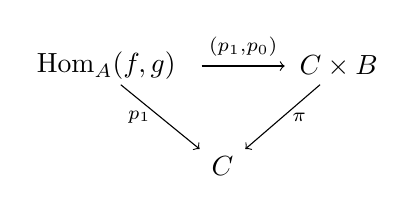
\begin{tikzpicture}[x=1.5em,y=1.5em]
  \node (H) at (0,1.4) {$\mathrm{Hom}_{A}(f,g)$};
  \node (CB) at (5.6,1.4) {$C\times B$};
  \node (C)  at (2.8,-1.0) {$C$};
  \draw[->] (2.3,1.4) -- node[above]{$\scriptstyle(p_{1},p_{0})$} (4.3,1.4);
  \draw[->] (0.35,0.95) -- node[left,pos=0.5]{$\scriptstyle p_{1}$} (2.25,-0.6);
  \draw[->] (5.15,0.95) -- node[right,pos=0.5]{$\scriptstyle\pi$} (3.35,-0.6);
\end{tikzpicture}
\end{center}
在 $\mathcal{K}_{/C}$ 中定义一条\trDiscreteCartesianFibration。
\end{enumerate}
\end{corollary}

\begin{proof}
我们从 (ii) 开始。由于
$p_{1}\colon\mathrm{Hom}_{A}(A,g)\twoheadrightarrow C$ 是
$p_{1}\colon A^{2}\twoheadrightarrow A$ 沿 $g$ 的一个\trPullback，我们可以利用%
\trCosmologicalFunctor{} $g^{*}\colon\mathcal{K}_{/A}\to\mathcal{K}_{/C}$ 把%
\cref{prop:domain-projection-sliced}的\trDiscreteCartesianFibration{}拉回成 $\mathcal{K}_{/C}$
中的一条\trDiscreteCartesianFibration：
\begin{center}
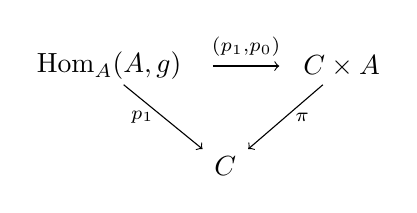
\begin{tikzpicture}[x=1.5em,y=1.5em]
  \node (H) at (0,1.4) {$\mathrm{Hom}_{A}(A,g)$};
  \node (CA) at (5.6,1.4) {$C\times A$};
  \node (C)  at (2.8,-1.0) {$C$};
  \draw[->] (2.5,1.4) -- node[above]{$\scriptstyle(p_{1},p_{0})$} (4.1,1.4);
  \draw[->] (0.35,0.95) -- node[left,pos=0.5]{$\scriptstyle p_{1}$} (2.25,-0.6);
  \draw[->] (5.15,0.95) -- node[right,pos=0.5]{$\scriptstyle\pi$} (3.35,-0.6);
\end{tikzpicture}
\end{center}
在 $\mathcal{K}_{/C}$ 中有一个\trPullback{}方块：
\begin{center}
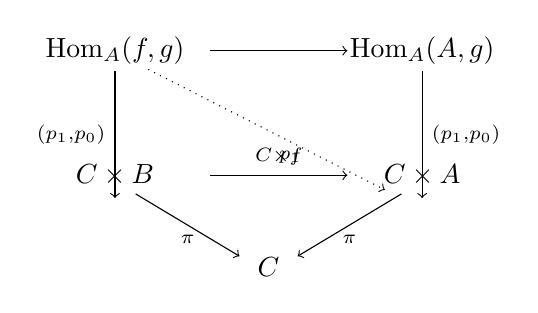
\begin{tikzpicture}[x=1.5em,y=1.5em]
  \node (Hfg) at (0,2.6) {$\mathrm{Hom}_{A}(f,g)$};
  \node (HAg) at (7.4,2.6) {$\mathrm{Hom}_{A}(A,g)$};
  \node (CB) at (0,-0.4) {$C\times B$};
  \node (CA) at (7.4,-0.4) {$C\times A$};
  \node (C)  at (3.7,-2.6) {$C$};
  \draw[->] (2.3,2.6) -- (5.6,2.6);
  \draw[->] (0,2.1) -- node[left]{$\scriptstyle(p_{1},p_{0})$} (0,-0.95);
  \draw[->] (7.4,2.1) -- node[right]{$\scriptstyle(p_{1},p_{0})$} (7.4,-0.95);
  \draw[->] (2.3,-0.4) -- node[above]{$\scriptstyle C\times f$} (5.6,-0.4);
  \node at (0.45,2.1) {$\scriptstyle\llcorner$};
  \draw[->,dotted] (0.8,2.15) -- node[below,pos=0.6]{$\scriptstyle p_{1}$} (6.5,-0.75);
  \draw[->] (0.5,-0.85) -- node[below,pos=0.5]{$\scriptstyle\pi$} (3.0,-2.35);
  \draw[->] (6.9,-0.85) -- node[below,pos=0.5]{$\scriptstyle\pi$} (4.4,-2.35);
\end{tikzpicture}
\end{center}
故由\cref{lem:discrete-pullback-stability}可知，该\trPullback{}也是一条\trDiscreteCartesianFibration。

利用 (ii)，我们现在可以证明 (i)。事实上，我们证明一个更一般的结论：若
\begin{center}
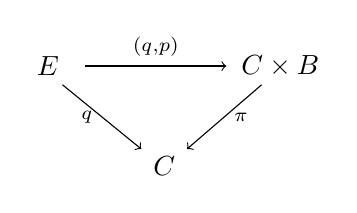
\begin{tikzpicture}[x=1.5em,y=1.5em]
  \node (E) at (0,1.4) {$E$};
  \node (CB) at (5.6,1.4) {$C\times B$};
  \node (C)  at (2.8,-1.0) {$C$};
  \draw[->] (0.9,1.4) -- node[above]{$\scriptstyle(q,p)$} (4.3,1.4);
  \draw[->] (0.35,0.95) -- node[left,pos=0.5]{$\scriptstyle q$} (2.25,-0.6);
  \draw[->] (5.15,0.95) -- node[right,pos=0.5]{$\scriptstyle\pi$} (3.35,-0.6);
\end{tikzpicture}
\end{center}
在 $\mathcal{K}_{/C}$ 中定义一条\trCartesianFibration，则
$p\colon E\twoheadrightarrow B$ 在 $\mathcal{K}$ 中定义一条%
\trCartesianFibration（见引理 7.1.1）。
在 $\mathcal{K}_{/C}$ 中应用定理 5.2.8(iii) 可知：函子
$\Delta_{(q,p)}=\Delta_{p}$ 容有一个 $C\times B$ 之上的\trRightAdjoint{} $r$：
\begin{center}
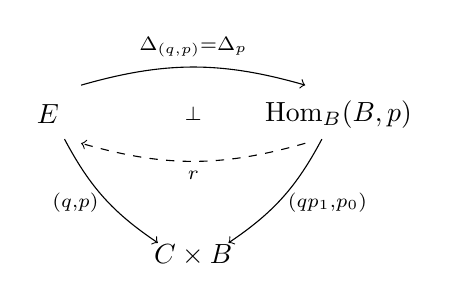
\begin{tikzpicture}[x=1.5em,y=1.5em]
  \node (E) at (0,1.6) {$E$};
  \node (H) at (7.0,1.6) {$\mathrm{Hom}_{B}(B,p)$};
  \draw[->] (0.8,2.3) to[bend left=16] node[above]{$\scriptstyle\Delta_{(q,p)}=\Delta_{p}$} (6.2,2.3);
  \node at (3.5,1.6) {$\scriptstyle\perp$};
  \draw[->,dashed] (6.2,0.9) to[bend left=16] node[below]{$\scriptstyle r$} (0.8,0.9);
  \node (CB) at (3.5,-1.8) {$C\times B$};
  \draw[->] (0.4,1.0) to[bend right=14] node[left,pos=0.55]{$\scriptstyle(q,p)$} (2.65,-1.5);
  \draw[->] (6.6,1.0) to[bend left=14] node[right,pos=0.55]{$\scriptstyle(qp_{1},p_{0})$} (4.35,-1.5);
\end{tikzpicture}
\end{center}
与 $\pi\colon C\times B\twoheadrightarrow B$ 复合，这一\trFiberedAdjunction{}便定义了一个
$B$ 之上的伴随。
这一次在 $\mathcal{K}$ 中应用定理 5.2.8(iii)，便使我们得以断定：
$p\colon E\twoheadrightarrow B$ 是一条\trCartesianFibration。
\end{proof}

注意，定义域投影 $p_{0}\colon\mathrm{Hom}_{A}(f,A)\twoheadrightarrow B$ 是
$p_{0}\colon A^{2}\twoheadrightarrow A$ 沿 $f\colon B\to A$ 的一个\trPullback，
故命题 5.2.4 与命题 5.2.9 蕴含这一函子是一条\trCartesianFibration；但
$p_{0}\colon\mathrm{Hom}_{A}(A,g)\twoheadrightarrow A$ 却不是
$p_{0}\colon A^{2}\twoheadrightarrow A$ 的类似拉回。这正是为得到 (i) 的结果
需要一个更迂回的论证的原因。

作为一个推论，我们终于可以引入\trDiscreteCartesianFibration{}的一个关键例子：

\begin{corollary}[由元素出发的定义域投影]\label{cor:domain-projection-from-element}
对任意元素 $b\colon 1\to B$，其定义域投影函子
\[
p_{0}\colon\mathrm{Hom}_{B}(B,b)\twoheadrightarrow B
\]
是一条\trDiscreteCartesianFibration。
\end{corollary}

\begin{proof}
由\cref{cor:comma-domain-projections}，
$p_{0}\colon\mathrm{Hom}_{B}(B,b)\twoheadrightarrow B$ 是一条%
\trCartesianFibration。离散性由\trTwoCellConservativity{}得出：若
\cellpair{X}{\mathrm{Hom}_{B}(B,b)}{f}{g}{\gamma}
是一个使 $p_{0}\gamma$ 为恒同的\trNaturalTransformation，则由于 $p_{1}\gamma$
也是恒同——此乃一个余定义域为\trTerminal{}∞-范畴的 2-胞腔——$\gamma$ 必定可逆。
\end{proof}


\subsection*{练习}

\begin{exercise}\label{ex:prove-discrete-isofibration-lemma}
证明\cref{lem:discrete-isofibration-characterizations}。
\end{exercise}

\begin{exercise}\label{ex:discreteness-exploration}
为探究\trDiscreteCartesianFibration{}的离散性：
\begin{enumerate}[label=(\roman*)]
\item 证明：$p_{0}\colon A^{2}\twoheadrightarrow A$ 是离散等价纤维化，当且仅当
$A$ 是一个离散的\trInfinityCategory。
\item 由\cref{cor:domain-projection-from-element}，对任何\trElement{}
$a\colon 1\to A$，$p_{0}\colon\mathrm{Hom}_{A}(A,a)\twoheadrightarrow A$
是一条\trDiscreteCartesianFibration。$\mathrm{Hom}_{A}(A,a)$ 必然是一个离散的%
\trInfinityCategory{}吗？
\end{enumerate}
\end{exercise}

\begin{exercise}\label{ex:alternate-proof-cartesian-functor}
利用定理 5.3.4 给出\cref{cor:square-into-discrete-cartesian}的另一个证明。
\end{exercise}
